\documentclass[a4paper]{article}\usepackage[]{graphicx}\usepackage[]{color}
%% maxwidth is the original width if it is less than linewidth
%% otherwise use linewidth (to make sure the graphics do not exceed the margin)
\makeatletter
\def\maxwidth{ %
  \ifdim\Gin@nat@width>\linewidth
    \linewidth
  \else
    \Gin@nat@width
  \fi
}
\makeatother

\definecolor{fgcolor}{rgb}{0.345, 0.345, 0.345}
\newcommand{\hlnum}[1]{\textcolor[rgb]{0.686,0.059,0.569}{#1}}%
\newcommand{\hlstr}[1]{\textcolor[rgb]{0.192,0.494,0.8}{#1}}%
\newcommand{\hlcom}[1]{\textcolor[rgb]{0.678,0.584,0.686}{\textit{#1}}}%
\newcommand{\hlopt}[1]{\textcolor[rgb]{0,0,0}{#1}}%
\newcommand{\hlstd}[1]{\textcolor[rgb]{0.345,0.345,0.345}{#1}}%
\newcommand{\hlkwa}[1]{\textcolor[rgb]{0.161,0.373,0.58}{\textbf{#1}}}%
\newcommand{\hlkwb}[1]{\textcolor[rgb]{0.69,0.353,0.396}{#1}}%
\newcommand{\hlkwc}[1]{\textcolor[rgb]{0.333,0.667,0.333}{#1}}%
\newcommand{\hlkwd}[1]{\textcolor[rgb]{0.737,0.353,0.396}{\textbf{#1}}}%
\let\hlipl\hlkwb

\usepackage{framed}
\makeatletter
\newenvironment{kframe}{%
 \def\at@end@of@kframe{}%
 \ifinner\ifhmode%
  \def\at@end@of@kframe{\end{minipage}}%
  \begin{minipage}{\columnwidth}%
 \fi\fi%
 \def\FrameCommand##1{\hskip\@totalleftmargin \hskip-\fboxsep
 \colorbox{shadecolor}{##1}\hskip-\fboxsep
     % There is no \\@totalrightmargin, so:
     \hskip-\linewidth \hskip-\@totalleftmargin \hskip\columnwidth}%
 \MakeFramed {\advance\hsize-\width
   \@totalleftmargin\z@ \linewidth\hsize
   \@setminipage}}%
 {\par\unskip\endMakeFramed%
 \at@end@of@kframe}
\makeatother

\definecolor{shadecolor}{rgb}{.97, .97, .97}
\definecolor{messagecolor}{rgb}{0, 0, 0}
\definecolor{warningcolor}{rgb}{1, 0, 1}
\definecolor{errorcolor}{rgb}{1, 0, 0}
\newenvironment{knitrout}{}{} % an empty environment to be redefined in TeX

\usepackage{alltt}
\usepackage[cm]{fullpage}
\usepackage{graphicx}
\usepackage{float}
\usepackage{caption}
\textwidth=18cm
\usepackage[backend=bibtex]{biblatex}



\IfFileExists{upquote.sty}{\usepackage{upquote}}{}
\begin{document}
\title{Sperry's supply-demand-loss model}
\author{Liam Langan}
\maketitle


\section{Introduction}
Sperry and Love (2015 (What plant hydraulics can tell us about responses to climate-change droughts)) developed a model where a supply function (transpiration rate) ($E$) (kg hr$^{-1}$ m$^{-2}$) is derived which calculates the potential rate/amount of water able to be supplied from the soil to the atmosphere. Transpiration ($E$) is influenced by the canopy sap pressure (p\_canopy) (MPa) via changes to the hydraulic conductance of the plant ($k$) (kg hr$^{-1}$ MPa$^{-1}$ m$^{-2}$). Hydraulic conductance of the plant ($k$) is the conductance when there is no difference in matric potential between the soil and the leaf.  

Below are parameters for the vulnerability-conductance curve,
\begin{knitrout}
\definecolor{shadecolor}{rgb}{0.969, 0.969, 0.969}\color{fgcolor}\begin{kframe}
\begin{alltt}
\hlcom{##-----------------------------------------------------------------------------------------------}
\hlstd{p50} \hlkwb{<-} \hlnum{2.5} \hlcom{# the matric potential where conductance is reduced by 50%}
\hlstd{k_max} \hlkwb{<-} \hlnum{8} \hlcom{# maximum plant conductance - this is a trait in aDGVM2}
\hlstd{res} \hlkwb{<-} \hlnum{1}\hlopt{/}\hlstd{k_max} \hlcom{# resistance is simply the inverse of conductance}
\hlstd{p_canopy} \hlkwb{<-} \hlkwd{seq}\hlstd{(}\hlnum{0.0}\hlstd{,} \hlnum{8}\hlstd{,} \hlkwc{length}\hlstd{=}\hlnum{1000}\hlstd{)}
\hlcom{# this assumes initial plant matric potential is the same as the soil matric potential}
\hlstd{predawn_soil_mat_pot} \hlkwb{<-} \hlkwd{seq}\hlstd{(}\hlnum{0}\hlstd{,}\hlnum{3}\hlstd{,} \hlkwc{length}\hlstd{=}\hlnum{5}\hlstd{)}
\hlstd{E_p_canopy} \hlkwb{<-} \hlkwd{matrix}\hlstd{(}\hlnum{0}\hlstd{,}\hlnum{0}\hlstd{,}\hlkwc{nrow}\hlstd{=}\hlnum{1000}\hlstd{,} \hlkwc{ncol}\hlstd{=}\hlnum{5}\hlstd{)} \hlcom{# matrix to hold the supply function values}

\hlcom{##-----------------------------------------------------------------------------------------------}
\hlcom{## make transpiration demand --------------------------------------------------------------------}
\hlcom{# Maximum stomatal conductance}
\hlcom{# (Sperry 2016, 2130 kg h^-1 m^-2) NOTE should be (kg h^-1 MPa^-1 m^-2) (12563.1 in Excel doc)}
\hlstd{Gmax} \hlkwb{<-} \hlnum{12563.1}
\hlstd{G} \hlkwb{<-} \hlkwd{rep}\hlstd{(Gmax,} \hlkwc{length}\hlstd{=}\hlnum{5}\hlstd{)}
\hlstd{D} \hlkwb{<-} \hlnum{0.5}\hlopt{*}\hlnum{0.001} \hlcom{#(Sperry 2016, leaf-to-air vapor pressure deficit 1 kPa)(0.001 converts to MPa) }
\hlcom{# NOTE VPD converstion from kPa to MPa isn't documented in Sperry, I'm doing it as it makes }
\hlcom{# sense and produces realistic amounts of transpirtational demand. }

\hlcom{# Pcrit, i.e. a matric potential we choose where we decide conductance is effectively zero. }
\hlcom{# Used this to get Ecrit, i.e. maximum transpiration beyond which leads to runaway cavitation  }
\hlstd{P_crit} \hlkwb{<-} \hlnum{6} \hlcom{# MPa - this is arbitrary and could be a plant trait. }
\hlcom{# In Sperry (2016) a P_crit cutoff is chosen (either very low conductance or }
\hlcom{# shallow slope of a tangent to the transpiration curve)}

\hlcom{# get maximum transpiration possible based on Pcrit and soil matric potential }
\hlstd{E_crit} \hlkwb{<-} \hlkwd{rep}\hlstd{(}\hlnum{0}\hlstd{,} \hlkwc{lenght}\hlstd{=}\hlnum{5}\hlstd{)} \hlcom{# maximum transpiration beyond which leads to runaway cavitation}
\hlstd{evap_demand} \hlkwb{<-} \hlkwd{rep}\hlstd{(}\hlnum{0}\hlstd{,} \hlkwc{lenght}\hlstd{=}\hlnum{5}\hlstd{)} \hlcom{# evaporative demand}
\end{alltt}
\end{kframe}
\end{knitrout}

with the the conductance vulnerability curve we use in aDGVM2, which is analagous to Sperry's curve, defined as:
\begin{knitrout}
\definecolor{shadecolor}{rgb}{0.969, 0.969, 0.969}\color{fgcolor}\begin{kframe}
\begin{alltt}
\hlstd{k_p_canopy} \hlkwb{<-} \hlkwa{function}\hlstd{(}\hlkwc{p_canopy}\hlstd{) \{ ((}\hlnum{1} \hlopt{-} \hlstd{(}\hlnum{1} \hlopt{/} \hlstd{(}\hlnum{1} \hlopt{+} \hlkwd{exp}\hlstd{(}\hlnum{3.0}\hlopt{*}\hlstd{(p50} \hlopt{-} \hlstd{p_canopy))))))} \hlopt{/} \hlstd{res \}}
\end{alltt}
\end{kframe}
\end{knitrout}
The transpiration rate is the integral of the vulnerability-conductance curve between the soil (pre-dawn) matric potential and (p\_canopy) and is calculated as follows: 

Here we get the slope of the line which is tangent to the tanspiration curve at any particulat water potential. This slope is the conductance at this water potential. 

We calculate the maximum transpiration beyond which leads to runaway cavitation $E_{crit}$ based on a matric potential we choose where we decide conductance is effectively zero $P_{crit}$. 
\begin{knitrout}
\definecolor{shadecolor}{rgb}{0.969, 0.969, 0.969}\color{fgcolor}\begin{kframe}
\begin{alltt}
\hlcom{##-----------------------------------------------------------------------------------------------}
\hlkwa{for}\hlstd{(j} \hlkwa{in} \hlnum{1}\hlopt{:}\hlnum{5}\hlstd{)}
\hlstd{\{}
  \hlstd{ffx} \hlkwb{<-} \hlkwd{integrate}\hlstd{(k_p_canopy, predawn_soil_mat_pot[j], P_crit )}
  \hlstd{E_crit[j]} \hlkwb{<-} \hlkwd{pmax}\hlstd{(}\hlnum{0}\hlstd{, ffx}\hlopt{$}\hlstd{value)}
  \hlstd{evap_demand[j]} \hlkwb{<-} \hlstd{G[j]}\hlopt{*}\hlstd{D}
  \hlkwa{if}\hlstd{(evap_demand[j]} \hlopt{>} \hlstd{E_crit[j]) evap_demand[j]} \hlkwb{<-} \hlstd{E_crit[j]} \hlcom{# demand = maximum supply}
\hlstd{\}}
\end{alltt}
\end{kframe}
\end{knitrout}

We then calculate the matric potential where evaporative demand is met
\begin{knitrout}
\definecolor{shadecolor}{rgb}{0.969, 0.969, 0.969}\color{fgcolor}\begin{kframe}
\begin{alltt}
\hlcom{## quick and dirty method to find the psi where demand is met. }
\hlstd{demand_met_at_sperry} \hlkwb{<-} \hlkwd{rep}\hlstd{(}\hlnum{0}\hlstd{,} \hlkwc{length}\hlstd{=}\hlnum{5}\hlstd{)}
\hlstd{psi_demand_met_at_sperry} \hlkwb{<-} \hlkwd{rep}\hlstd{(}\hlnum{0}\hlstd{,} \hlkwc{length}\hlstd{=}\hlnum{5}\hlstd{)}
\hlstd{demand_met_at_slope_sperry} \hlkwb{<-} \hlkwd{rep}\hlstd{(}\hlnum{0}\hlstd{,} \hlkwc{length}\hlstd{=}\hlnum{5}\hlstd{)}
\hlstd{loss_function_sperry} \hlkwb{<-} \hlkwd{rep}\hlstd{(}\hlnum{0}\hlstd{,} \hlkwc{length}\hlstd{=}\hlnum{5}\hlstd{)}
\hlstd{regulated_transpiration} \hlkwb{<-} \hlkwd{rep}\hlstd{(}\hlnum{0}\hlstd{,} \hlkwc{length}\hlstd{=}\hlnum{5}\hlstd{)}
\hlstd{regulated_leaf_psi} \hlkwb{<-} \hlkwd{rep}\hlstd{(}\hlnum{0}\hlstd{,} \hlkwc{length}\hlstd{=}\hlnum{5}\hlstd{)}

\hlcom{##-----------------------------------------------------------------------------------------------}
\hlcom{##-----------------------------------------------------------------------------------------------}

\hlcom{#max regulation is the point where delta P hits its maximum, held constant at max once max passed}
\hlstd{G} \hlkwb{<-} \hlkwd{matrix}\hlstd{(Gmax, Gmax, ,}\hlkwc{nrow}\hlstd{=}\hlnum{1000}\hlstd{,} \hlkwc{ncol}\hlstd{=}\hlnum{5}\hlstd{)}

\hlstd{psi_1} \hlkwb{<-} \hlkwd{matrix}\hlstd{(}\hlnum{0}\hlstd{,}\hlnum{0}\hlstd{,}\hlkwc{nrow}\hlstd{=}\hlnum{1000}\hlstd{,} \hlkwc{ncol}\hlstd{=}\hlnum{5}\hlstd{)}\hlcom{#}
\hlstd{slope_demand} \hlkwb{<-} \hlkwd{matrix}\hlstd{(}\hlnum{0}\hlstd{,}\hlnum{0}\hlstd{,}\hlkwc{nrow}\hlstd{=}\hlnum{1000}\hlstd{,} \hlkwc{ncol}\hlstd{=}\hlnum{5}\hlstd{)}
\hlstd{loss_fun_sp_gs} \hlkwb{<-} \hlkwd{matrix}\hlstd{(}\hlnum{0}\hlstd{,}\hlnum{0}\hlstd{,}\hlkwc{nrow}\hlstd{=}\hlnum{1000}\hlstd{,} \hlkwc{ncol}\hlstd{=}\hlnum{5}\hlstd{)}
\hlstd{reg_leaf_psi} \hlkwb{<-} \hlkwd{matrix}\hlstd{(}\hlnum{0}\hlstd{,}\hlnum{0}\hlstd{,}\hlkwc{nrow}\hlstd{=}\hlnum{1000}\hlstd{,} \hlkwc{ncol}\hlstd{=}\hlnum{5}\hlstd{)}

\hlstd{regulated_trans} \hlkwb{<-} \hlkwd{matrix}\hlstd{(}\hlnum{0}\hlstd{,}\hlnum{0}\hlstd{,}\hlkwc{nrow}\hlstd{=}\hlnum{1000}\hlstd{,} \hlkwc{ncol}\hlstd{=}\hlnum{5}\hlstd{)}
\hlstd{regulated_Gs} \hlkwb{<-} \hlkwd{matrix}\hlstd{(}\hlnum{0}\hlstd{,}\hlnum{0}\hlstd{,}\hlkwc{nrow}\hlstd{=}\hlnum{1000}\hlstd{,} \hlkwc{ncol}\hlstd{=}\hlnum{5}\hlstd{)}

\hlstd{non_regulated_Gs} \hlkwb{<-} \hlkwd{matrix}\hlstd{(}\hlnum{0}\hlstd{,}\hlnum{0}\hlstd{,}\hlkwc{nrow}\hlstd{=}\hlnum{1000}\hlstd{,} \hlkwc{ncol}\hlstd{=}\hlnum{5}\hlstd{)}

\hlstd{max_slo_sp} \hlkwb{<-} \hlkwd{rep}\hlstd{(}\hlnum{0}\hlstd{,} \hlkwc{length}\hlstd{=}\hlnum{5}\hlstd{)}

\hlkwa{for}\hlstd{(j} \hlkwa{in} \hlnum{1}\hlopt{:}\hlnum{5}\hlstd{)}
\hlstd{\{}

  \hlstd{max_slo_sp[j]} \hlkwb{<-} \hlkwd{k_p_canopy}\hlstd{(predawn_soil_mat_pot[j])}

  \hlkwa{for}\hlstd{(i} \hlkwa{in} \hlnum{1}\hlopt{:}\hlnum{1000}\hlstd{)}
  \hlstd{\{}
   \hlstd{psi_1[,j]} \hlkwb{<-} \hlkwd{seq}\hlstd{(}\hlnum{0}\hlstd{,} \hlkwd{max}\hlstd{(p_canopy),} \hlkwc{length}\hlstd{=}\hlnum{1000}\hlstd{)} \hlcom{#psi_leaf[i]}
   \hlstd{slope_demand[i,j]} \hlkwb{<-} \hlkwd{k_p_canopy}\hlstd{(psi_1[i,j])}

   \hlstd{ffx} \hlkwb{<-} \hlkwd{integrate}\hlstd{(k_p_canopy, predawn_soil_mat_pot[j], psi_1[i,j] )}
   \hlstd{E_p_canopy[i,j]} \hlkwb{<-} \hlkwd{pmax}\hlstd{(}\hlnum{0}\hlstd{, ffx}\hlopt{$}\hlstd{value)}
   \hlstd{non_regulated_Gs[i,j]} \hlkwb{<-} \hlstd{E_p_canopy[i,j]}\hlopt{/}\hlstd{D}
   \hlcom{# E = G*VPD ---- G = E/VPD (VPD=1, 0.001 transforms to MPa)}

   \hlstd{loss_fun_sp_gs[i,j]} \hlkwb{<-} \hlstd{slope_demand[i,j]} \hlopt{/} \hlstd{max_slo_sp[j]}

   \hlkwa{if}\hlstd{(i}\hlopt{==}\hlnum{1}\hlstd{) reg_leaf_psi[i,j]} \hlkwb{<-} \hlkwd{pmax}\hlstd{(}\hlnum{0}\hlstd{, ((psi_1[i,j]} \hlopt{-} \hlstd{predawn_soil_mat_pot[j])}
                                          \hlopt{*}\hlstd{loss_fun_sp_gs[i,j]))}

   \hlkwa{if}\hlstd{(i}\hlopt{>}\hlnum{1}\hlstd{)}
   \hlstd{\{}
     \hlstd{reg_leaf_psi[i,j]} \hlkwb{<-} \hlkwd{pmax}\hlstd{(}\hlnum{0}\hlstd{,} \hlkwd{pmax}\hlstd{(reg_leaf_psi[i}\hlopt{-}\hlnum{1}\hlstd{,j],}
                                  \hlstd{((psi_1[i,j]} \hlopt{-} \hlstd{predawn_soil_mat_pot[j])}\hlopt{*}\hlstd{loss_fun_sp_gs[i,j])))}
   \hlstd{\}}

   \hlstd{ffx} \hlkwb{<-} \hlkwd{integrate}\hlstd{(k_p_canopy, predawn_soil_mat_pot[j],}
                    \hlstd{predawn_soil_mat_pot[j]} \hlopt{+} \hlstd{reg_leaf_psi[i,j])}
   \hlstd{regulated_trans[i,j]} \hlkwb{<-} \hlkwd{pmax}\hlstd{(}\hlnum{0}\hlstd{, ffx}\hlopt{$}\hlstd{value)}
   \hlstd{regulated_Gs[i,j]} \hlkwb{<-} \hlstd{regulated_trans[i,j]}\hlopt{/}\hlstd{D} \hlcom{# E=G*D -- G=E/D (D=1, 0.001 transforms to MPa)}
   \hlstd{G[i,j]} \hlkwb{<-} \hlstd{G[i,j]}\hlopt{*}\hlstd{loss_fun_sp_gs[i,j]}
  \hlstd{\}}
\hlstd{\}}

\hlstd{demand_place_holder} \hlkwb{<-} \hlkwd{rep}\hlstd{(}\hlnum{0}\hlstd{,} \hlkwc{length}\hlstd{=}\hlnum{5}\hlstd{)}
\hlstd{supply_limit_place_holder} \hlkwb{<-} \hlkwd{rep}\hlstd{(}\hlnum{0}\hlstd{,} \hlkwc{length}\hlstd{=}\hlnum{5}\hlstd{)}
\hlstd{min_diff_place_holder} \hlkwb{<-} \hlkwd{rep}\hlstd{(}\hlnum{0}\hlstd{,} \hlkwc{length}\hlstd{=}\hlnum{5}\hlstd{)}
\hlstd{supply_place_holder} \hlkwb{<-} \hlkwd{rep}\hlstd{(}\hlnum{0}\hlstd{,} \hlkwc{length}\hlstd{=}\hlnum{5}\hlstd{)}


\hlkwa{for}\hlstd{(i} \hlkwa{in} \hlnum{1}\hlopt{:}\hlnum{5}\hlstd{)}
\hlstd{\{}
    \hlstd{a} \hlkwb{<-}\hlkwd{which}\hlstd{(E_p_canopy[,i]} \hlopt{>=} \hlstd{evap_demand[i])}
    \hlstd{demand_place_holder[i]} \hlkwb{<-}\hlstd{a[}\hlnum{2}\hlstd{]}

    \hlstd{min_diff} \hlkwb{<-} \hlstd{regulated_trans[,i]} \hlopt{-} \hlstd{E_p_canopy[demand_place_holder[i]]}
    \hlstd{min_diff_max} \hlkwb{<-} \hlkwd{which}\hlstd{(min_diff} \hlopt{==} \hlkwd{max}\hlstd{(min_diff))}
    \hlstd{supply_limit_place_holder[i]} \hlkwb{<-} \hlstd{min_diff_max[}\hlnum{1}\hlstd{]}

    \hlstd{abs_min_diff} \hlkwb{<-} \hlkwd{abs}\hlstd{(min_diff)}
    \hlstd{abs_min_diff} \hlkwb{<-} \hlkwd{which}\hlstd{(abs_min_diff} \hlopt{==} \hlkwd{min}\hlstd{(abs_min_diff))}
    \hlstd{supply_place_holder[i]} \hlkwb{<-} \hlstd{abs_min_diff[}\hlnum{1}\hlstd{]}
\hlstd{\}}
\end{alltt}
\end{kframe}
\end{knitrout}

%\begin(figure)
\begin{centering}
\begin{knitrout}
\definecolor{shadecolor}{rgb}{0.969, 0.969, 0.969}\color{fgcolor}\begin{figure}
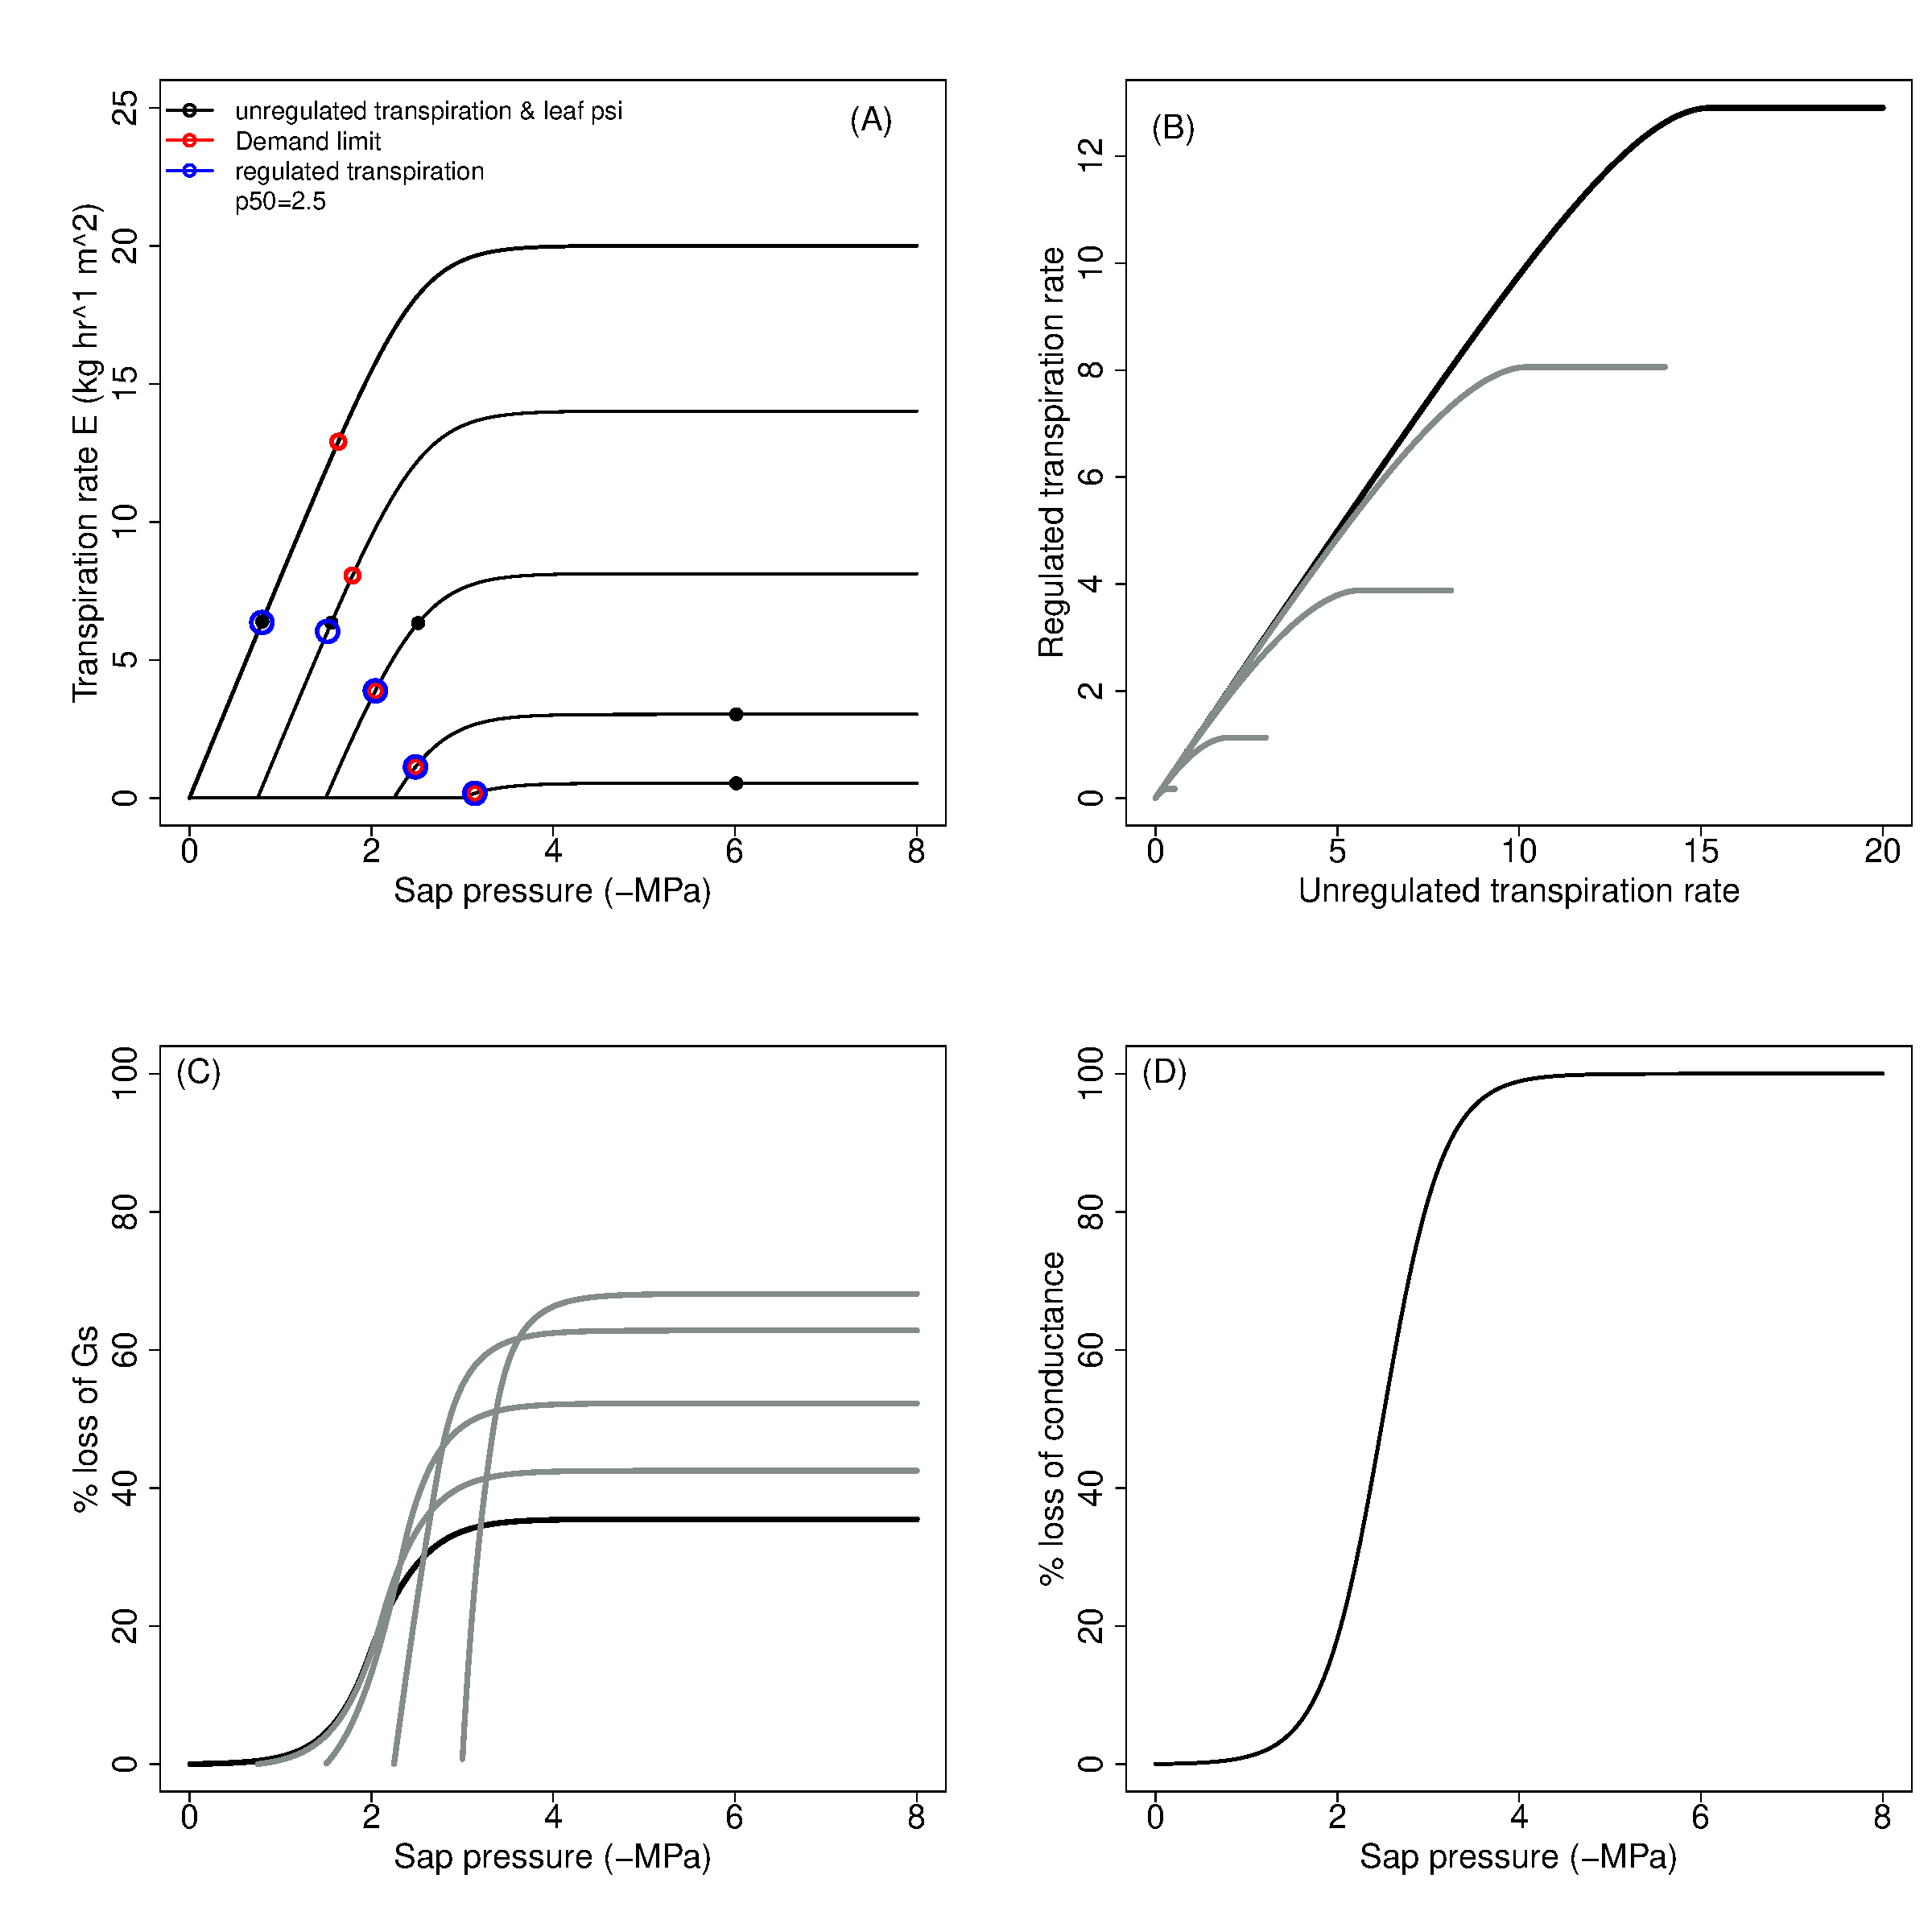
\includegraphics[width=\maxwidth]{figure/unnamed-chunk-7-1} \caption{\label{fig:figs}(A) Unregulated and regulated transpiration with supply demand limit. Where curves intersect the x-axis indicate the predawn/soil matric potential. (B) Regulated vs unregulated transpiration. the differing curves represent the responses for the differing predawn/soil matric potentials in (A). (C) Loss of stomatal conductance NOTE I haven't worked out how Sperry is producing his Fig.4 in Sperry and Love (2015). The differing curves correspond to the differing predawn/soil matric potentials in (A). (D) percentage loss of conductance.}\label{fig:unnamed-chunk-7}
\end{figure}


\end{knitrout}
\end{centering}

%\caption{Plot of 1:10 and a bar plot beside it in a figure that is 4x6 inches}
%\end(figure)

From Sperry (2016) "Mathematically, ΔP rises to a maximum before decreasing back to zero as E 0 increases to Ecrit. This decline in ΔP is unrealis- tic (Saliendra et al., 1995), so it is assumed that ΔP saturates at its maximum as E 0 increases. Eqn 5 expresses the outcome that xylem pressure is regulated in proportion to the damage caused by taking no action. (4) The regulated E corresponding to ΔP is determined from the supply function. (5) The G is solved from E/D to determine how much it is reduced below Gmax. The model does not partition G into stomatal vs boundary layer com- ponents, but G is controlled by stomatal regulation. Cuticular water loss is assumed to be zero." I was unsure what Sperry ment with $\Delta P$ saturates however examining Fig.1B one can see the regulated response is too extreme. Plotting the regulated leaf matric potential against the demand defined matiric reveals that the regulated leaf matric potential reaches a maximum and then decreases. Fixing the regulated leaf matric potential to its maximum value once it has passed this value solves this issue. The next issue to solve is how sperry is calculating his percentage loss of stomatal conductance.  


%begin{centering}
%<<fig.width=16, echo=FALSE, fig.height=8, ,fig.cap="\\label{fig:figs}Regulated leaf matric potential against the demand defined matiric potential.">>==
%par(mfrow=c(1,1), mar=c(7,8,4,1))
%plot(psi_canopy, regulated_leaf_psi[,1], type="l", ylab="Delta P ", xlab="Sap pressure (-MPa)", cex.lab=2.0, cex.axis=2.0,lwd=2.5)
%text(4.5, 7.8,"(A)", cex=2)

%@
%\end{centering}


\end{document}











